\fichetrue
\proftrue
\tdfalse
\coursfalse



\def\xxnumchapitre{Chapitre 2 \vspace{.2cm}}
\def\xxchapitre{\hspace{.12cm} Définitions préliminaires et détermination des performances}
\def\xxYCartouche{-2.25cm}
\def\xxposongletx{2}
\def\xxposonglettext{1.45}
\def\xxposonglety{19}%16

\def\xxonglet{Cy 01 -- Ch 2}

\def\xxactivite{Fiche}


\def\xxpied{%
Cycle 01 -- Modéliser le comportement des systèmes multiphysiques\\
Ch 2 -- \xxactivite%
}

\setcounter{secnumdepth}{5}
%---------------------------------------------------------------------------

\iflivret
\input{../../../Style/pagegarde_Fiche}
\else
\pagestyle{empty}


%%%%%%%% PAGE DE GARDE COURS
\ifcours
\begin{tikzpicture}[remember picture,overlay]
\node at (current page.north west)
{\begin{tikzpicture}[remember picture,overlay]
\node[anchor=north west,inner sep=0pt] at (0,0) {\includegraphics[width=\paperwidth]{\thechapterimage}};
\draw[anchor=west] (-2cm,-8cm) node [line width=2pt,rounded corners=15pt,draw=ocre,fill=white,fill opacity=0.6,inner sep=40pt]{\strut\makebox[22cm]{}};
\draw[anchor=west] (1cm,-8cm) node {\huge\sffamily\bfseries\color{black} %
\begin{minipage}{1cm}
\rotatebox{90}{\LARGE\sffamily\textsc{\color{ocre}\textbf{\xxnumpartie}}}
\end{minipage} \hfill
\begin{minipage}[c]{14cm}
\begin{titrepartie}
\begin{flushright}
\renewcommand{\baselinestretch}{1.1} 
\Large\sffamily\textsc{\textbf{\xxpartie}}
\renewcommand{\baselinestretch}{1} 
\end{flushright}
\end{titrepartie}
\end{minipage} \hfill
\begin{minipage}[c]{3.5cm}
{\large\sffamily\textsc{\textbf{\color{ocre} \discipline}}}
\end{minipage} 
 };
\end{tikzpicture}};
\end{tikzpicture}


\begin{tikzpicture}[overlay]
\node[shape=rectangle, 
      rounded corners = .25 cm,
	  draw= ocre,
	  line width=2pt, 
	  fill = ocre!10,
	  minimum width  = 2.5cm,
	  minimum height = 3cm,] at (18cm,0) {};
\node at (17.7cm,0) {\rotatebox{90}{\textbf{\Large\color{ocre}{\classe}}}};
%{};
\end{tikzpicture}

\vspace{3.5cm}

\begin{tikzpicture}[remember picture,overlay]
\draw[anchor=west] (-2cm,-6cm) node {\huge\sffamily\bfseries\color{black} %
\begin{minipage}{2cm}
\begin{center}
\LARGE\sffamily\textsc{\color{ocre}\textbf{\xxactivite}}
\end{center}
\end{minipage} \hfill
\begin{minipage}[c]{15cm}
\begin{titrechapitre}
\renewcommand{\baselinestretch}{1.1} 
\Large\sffamily\textsc{\textbf{\xxnumchapitre}}

\Large\sffamily\textsc{\textbf{\xxchapitre}}
\vspace{.5cm}

\renewcommand{\baselinestretch}{1} 
\normalsize\normalfont
\xxcompetences
\end{titrechapitre}
\end{minipage}  };
\end{tikzpicture}
\vfill

\begin{flushright}
\begin{minipage}[c]{.3\linewidth}
\begin{center}
\xxfigures
\end{center}
\end{minipage}\hfill
\begin{minipage}[c]{.6\linewidth}
\startcontents
\printcontents{}{1}{}
\end{minipage}
\end{flushright}

\begin{tikzpicture}[remember picture,overlay]
\draw[anchor=west] (4.5cm,-.7cm) node {
\begin{minipage}[c]{.2\linewidth}
\begin{flushright}

\includegraphics[width=2cm]{png/logoCC}
\end{flushright}
\end{minipage}
\begin{minipage}[c]{.2\linewidth}
\textsl{\xxauteur} \\
\textsl{\classe}
\end{minipage}
 };
\end{tikzpicture}
\newpage
\pagestyle{fancy}

\newpage
\pagestyle{fancy}

\else
\fi


%%%%%%%% PAGE DE GARDE TD
\iftd
%\begin{tikzpicture}[remember picture,overlay]
%\node at (current page.north west)
%{\begin{tikzpicture}[remember picture,overlay]
%\draw[anchor=west] (-2cm,-3.25cm) node [line width=2pt,rounded corners=15pt,draw=ocre,fill=white,fill opacity=0.6,inner sep=40pt]{\strut\makebox[22cm]{}};
%\draw[anchor=west] (1cm,-3.25cm) node {\huge\sffamily\bfseries\color{black} %
%\begin{minipage}{1cm}
%\rotatebox{90}{\LARGE\sffamily\textsc{\color{ocre}\textbf{\xxnumpartie}}}
%\end{minipage} \hfill
%\begin{minipage}[c]{13.5cm}
%\begin{titrepartie}
%\begin{flushright}
%\renewcommand{\baselinestretch}{1.1} 
%\Large\sffamily\textsc{\textbf{\xxpartie}}
%\renewcommand{\baselinestretch}{1} 
%\end{flushright}
%\end{titrepartie}
%\end{minipage} \hfill
%\begin{minipage}[c]{3.5cm}
%{\large\sffamily\textsc{\textbf{\color{ocre} \discipline}}}
%\end{minipage} 
% };
%\end{tikzpicture}};
%\end{tikzpicture}

%%%%%%%%%% PAGE DE GARDE TD %%%%%%%%%%%%%%%
%\begin{tikzpicture}[overlay]
%\node[shape=rectangle, 
%      rounded corners = .25 cm,
%	  draw= ocre,
%	  line width=2pt, 
%	  fill = ocre!10,
%	  minimum width  = 2.5cm,
%	  minimum height = 2.5cm,] at (18.5cm,0) {};
%\node at (17.7cm,0) {\rotatebox{90}{\textbf{\Large\color{ocre}{\classe}}}};
%%{};
%\end{tikzpicture}

% PARTIE ET CHAPITRE
%\begin{tikzpicture}[remember picture,overlay]
%\draw[anchor=west] (-1cm,-2.1cm) node {\large\sffamily\bfseries\color{black} %
%\begin{minipage}[c]{15cm}
%\begin{flushleft}
%\xxnumchapitre \\
%\xxchapitre
%\end{flushleft}
%\end{minipage}  };
%\end{tikzpicture}

% Bandeau titre exo
\begin{tikzpicture}[remember picture,overlay]
\draw[anchor=west] (-2cm,-6cm) node {\huge\sffamily\bfseries\color{black} %
\begin{minipage}{5cm}
\begin{center}
\LARGE\sffamily\color{ocre}\textbf{\textsc{\xxactivite}}

\begin{center}
\xxfigures
\end{center}

\end{center}
\end{minipage} \hfill
\begin{minipage}[c]{12cm}
\begin{titrechapitre}
\renewcommand{\baselinestretch}{1.1} 
\large\sffamily\textbf{\textsc{\xxtitreexo}}

\small\sffamily{\textbf{\textit{\color{black!70}\xxsourceexo}}}
\vspace{.5cm}

\renewcommand{\baselinestretch}{1} 
\normalsize\normalfont
\xxcompetences
\end{titrechapitre}
\end{minipage}  };
\end{tikzpicture}

\else
\fi


%%%%%%%% PAGE DE GARDE FICHE
\iffiche
\begin{tikzpicture}[remember picture,overlay]
\node at (current page.north west)
{\begin{tikzpicture}[remember picture,overlay]
\draw[anchor=west] (-2cm,-3.25cm) node [line width=2pt,rounded corners=15pt,draw=ocre,fill=white,fill opacity=0.6,inner sep=40pt]{\strut\makebox[22cm]{}};
\draw[anchor=west] (1cm,-3.25cm) node {\huge\sffamily\bfseries\color{black} %
\begin{minipage}{1cm}
\rotatebox{90}{\LARGE\sffamily\textsc{\color{ocre}\textbf{\xxnumpartie}}}
\end{minipage} \hfill
\begin{minipage}[c]{14cm}
\begin{titrepartie}
\begin{flushright}
\renewcommand{\baselinestretch}{1.1} 
\large\sffamily\textsc{\textbf{\xxpartie} \\} 

\vspace{.2cm}

\normalsize\sffamily\textsc{\textbf{\xxnumchapitre -- \xxchapitre}}
\renewcommand{\baselinestretch}{1} 
\end{flushright}
\end{titrepartie}
\end{minipage} \hfill
\begin{minipage}[c]{3.5cm}
{\large\sffamily\textsc{\textbf{\color{ocre} \discipline}}}
\end{minipage} 
 };
\end{tikzpicture}};
\end{tikzpicture}


\begin{tikzpicture}[overlay]
\node[shape=rectangle, 
      rounded corners = .25 cm,
	  draw= ocre,
	  line width=2pt, 
	  fill = ocre!10,
	  minimum width  = 2.5cm,
%	  minimum height = 2.5cm,] at (18.5cm,0.5cm) {};
	  minimum height = 2.5cm,] at (18.5cm,0cm) {};
\node at (17.7cm,0) {\rotatebox{90}{\textsf{\textbf{\large\color{ocre}{\classe}}}}};
%{};
\end{tikzpicture}



\else
\fi



\fi
\vspace{.5cm}
\pagestyle{fancy}
\thispagestyle{plain}
\setcounter{section}{0}


\section{Définitions}



\begin{defi}\textbf{Informations analogiques et numériques} ~\\
\begin{itemize}[label=\ding{112},font=\color{bleuxp}] 
\item Une information analogique peut prendre, de manière continue, toutes les valeurs
possibles dans un intervalle donné. Un signal analogique peut être représenté
par une courbe continue. Les grandeurs physiques (température, vitesse,
position, tension, ...) sont des informations analogiques.

\item Une information numérique sous la forme d'un mot binaire est constituée de
plusieurs bits (variables binaires 0/1). Cette information numérique est en
général issue d'un traitement (échantillonnage et codage) d'une information
analogique. On parle de conversion analogique numérique (CAN).
\end{itemize}
\end{defi}

\begin{center}
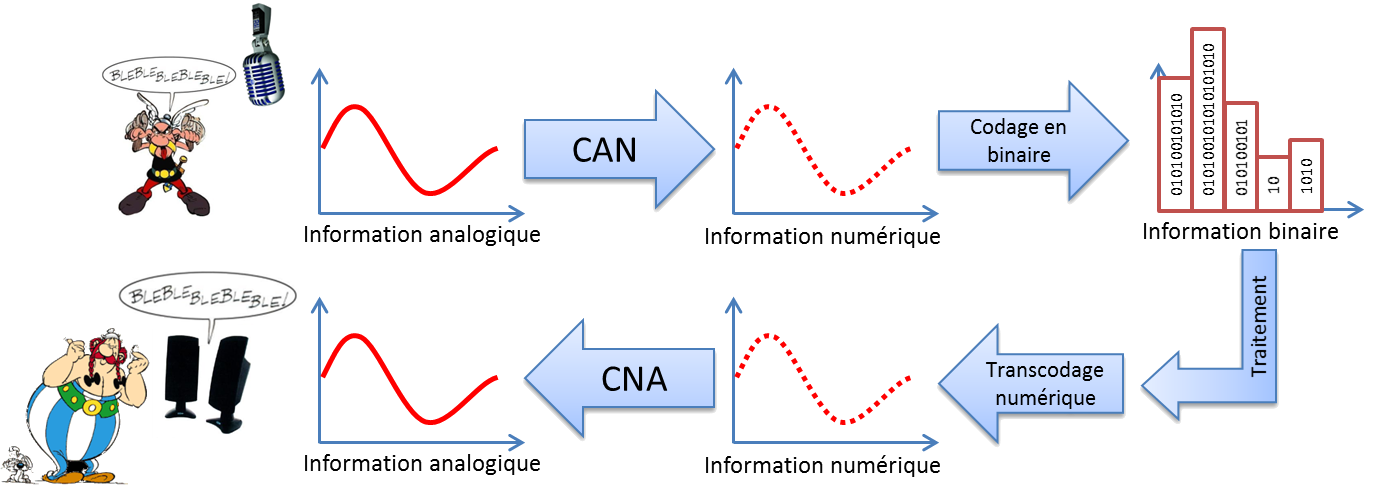
\includegraphics[width=.8\textwidth]{CAN_CNA}

\end{center}



\begin{defi}\textbf{Systèmes automatiques ou asservis} ~\\

\noindent\begin{minipage}[c]{11cm}
Un système asservi est commandé par \textbf{une (ou des) entrée(s)} qu'il
transforme en \textbf{grandeur(s) de sortie}.
Les entrées sont de deux types : 
\begin{itemize}
 \item la loi de consigne $e(t)$ est une grandeur de commande qui est
modifiable;
\item la perturbation : c'est une entrée parasite qui nuit au bon
fonctionnement du système. On ne peut pas modifier les perturbations.
\end{itemize}
\end{minipage} \hfill
\begin{minipage}[c]{5cm}
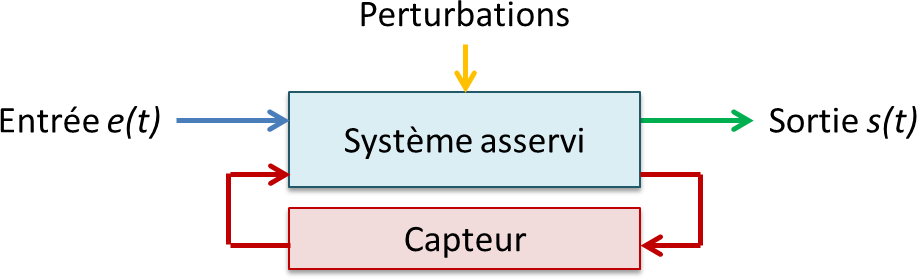
\includegraphics[width=5cm]{Systeme_Asservi}
\end{minipage}

\noindent
La sortie $s(t)$ est une grandeur \textbf{observable} (par des capteurs) qui
permet de juger de la qualité de la tâche accomplie.


\end{defi} 


\begin{defi}\textbf{Systèmes suiveurs et régulateurs} ~\\
\begin{itemize}[label=\ding{112},font=\color{bleuxp}] 
\item Pour un système suiveur la consigne $e(t)$ fluctue au cours du temps. Le système doit faire son possible pour qu'à chaque instant la cible soit suivie.
\item Pour un système régulateur la consigne $e(t)$ est constante. Les perturbations font varier la position du système. Il doit donc de façon automatique revenir à la position commandée.
\end{itemize}
\end{defi}


\begin{center}
%\includestandalone{suiveur}
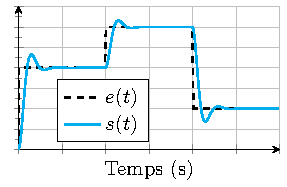
\includegraphics{suiveur}
\hspace{2cm}
%\includestandalone{regulateur}
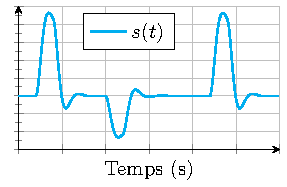
\includegraphics{regulateur}
\end{center}



\section{Performance des systèmes -- Critères graphiques}
\begin{defi}\textbf{Précision en position -- Écart statique $\varepsilon_S$}

Le système est piloté par un échelon. On définit alors l'écart statique $\varepsilon_S$ comme l'écart entre la consigne fixe et la réponse $s(t)$ en régime permanent.
\end{defi}

\begin{defi}\textbf{Précision en vitesse $\varepsilon_V$}

Encore appelé écart de traînage ou écart de poursuite, il représente la différence entre une consigne variable de type rampe et la réponse en régime permanent. 
\end{defi}

\begin{defi}\textbf{Rapidité}

La rapidité est caractérisée par le temps que met le système à réagir à une
variation brusque de la grandeur d'entrée (temps de réponse). Cette notion est
fortement liée à la notion de précision dynamique.
\end{defi}

\begin{methode}\textbf{Détermination du temps de réponse à $n\%$} (En pratique $n=5$).\\

\begin{enumerate}
 \item Tracer sur le même graphe la consigne $e(t)$ et la réponse du système
$s(t)$.
\item Tracer la droite correspondant à la valeur asymptotique de $s(t)$.
\item Tracer la bande correspondant à une variation de $\pm n\%$ de la valeur
asymptotique.
\item Relever la dernière valeur à partir de laquelle $s(t)$ coupe la bande et
n'en sort plus.
\end{enumerate}
\end{methode}


\begin{center}
%\includestandalone{perf}
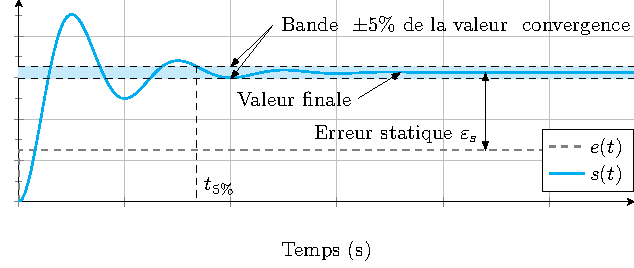
\includegraphics{perf}
\hfill
%\includestandalone{rampe}
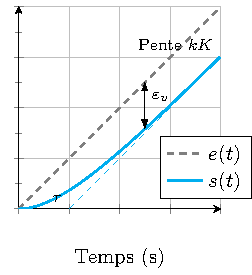
\includegraphics{rampe}
\end{center}

\begin{defi}\textbf{Stabilité}

La stabilité traduit la propriété de convergence temporelle asymptotique vers
un état d'équilibre. 
\end{defi}



